\section{Leaching}
-popis, příčiny a předcházení jevu, význam intermetalických sloučenin v pájeném spoji

\subsection{Popis}
Negativní jev, který nastává během procesu pájení na tlustou vrstvu. Jedná se o rozpouštění pájeného materiálu (kovu) do roztavené pájky. Rychlost rozpouštění kovu v pájce je ovlivněna několika faktory. Prvním je velikost teploty a délka procesu
pájení. Druhým je použitý materiál pájecí plošky, tzn. měď, stříbro, zlato, atp., a zvolená pájecí slitina. Teplotu v pájecím procesu nemůžeme příliš ovlivnit, ale můžeme ovlivnit použité materiály. Rychlost rozpouštění pájecí plošky je závislá právě na zvolené kombinaci materiálů pájky a pájecí plošky. V následujících příkladech jsou ukázány vlivy použitých materiálů, z pohledu pájecí slitiny v prvním případě a z pohledu pájecí plošky ve druhém případě.

\textbf{1.} Přidáním stříbra do pájecí slitiny snižujeme rozpouštění stříbrné pájecí plošky do pájky. Pokud
se v pájce vyskytuje přibližně jedno procento india, docílí se tím sníženého rozpouštění zlata do pájky.\\
\textbf{2.} Obsah až 20 \% paládia v tlustovrstvé pájecí plošce snižuje její rozpouštění v pájecí slitině.
Levnější metodou je galvanické vytvoření niklové vrstvy na pájecí plošce s tenkou vrstvou pájecí slitiny.

V praxi většinou není nutné řešit kompatibilitu použitých materiálu, tzn. pájecí slitiny a tlusté vrstvy, jelikož výrobce tlustovrstvé vodivé pasty udává v katalogovém listu možnost pájitelnosti a také je zde uvedena minimálně jedna kompatibilní pájecí slitina. Leaching prakticky nastává i u desek plošných spojů, avšak vzhledem k použité mědi, jako materiálu pájecích plošek, nedochází k rozpouštění v takové míře a rychlosti, jako je tomu u tlustých vrstev. Také je nutné brát v potaz strukturu a tloušťku pájecí plošky.

\subsection{Zlato}
Zlaté vodiče mají v tlustovrstvých obvodech a strukturách široké uplatnění. Nejčastěji se využívají v aplikacích, u kterých je vyžadovaný vysoký stupeň spolehlivosti jako např. ve vojenských a medicínských aplikacích.

Pokud chceme dosáhnout požadované spolehlivosti, musí být montážní procesy v případě
zlatých vodičů voleny s velkou opatrností (leaching).
\subsubsection{Něco navíc ke zlatu}
Zlato a cín vytváří křehkou intermetalickou sloučeninu s velkým elektrickým odporem.

V případě použití SnPb slitin je třeba použít jako materiál plošek zlato ve slitině s platinou (Pt) nebo paládiem (Pd) - minimalizace leachingu a vzniku nežádoucích intermetalických
sloučenin.

Zlato vytváří intermetalické sloučeniny také s hliníkem (Al), který se využívá pro připojování polovodičových struktur např. pomocí mikrodrátkových propojů (wire bonding -
kontaktování).

Difuzní koeficient hliníku do zlata je mnohem větší než zlata do hliníku - míra difuze rapidně
vzůrstá s teplotou.

Tento jev se může stát významným např. také na rozhraní Au - Al při kontaktování (jak na
čip, tak na TLV plošku). Kdy může např. hliník difundovat do zlatého drátku a přitom za
sebou zanechávat přázdná místa (Kirkendall voids), která oslabují pevnost spoje a zvyšují jeho odpor. Tento jev se výrazně zvyšuje nad teplotou 170 °C a představuje riziko z pohledu
spolehlivosti.

Přídavek paládia do zlata výrazným způsobem snižuje míru difuze a tím zvyšuje spolehlivost
spoje.

\begin{figure}[h]
   \begin{center}
     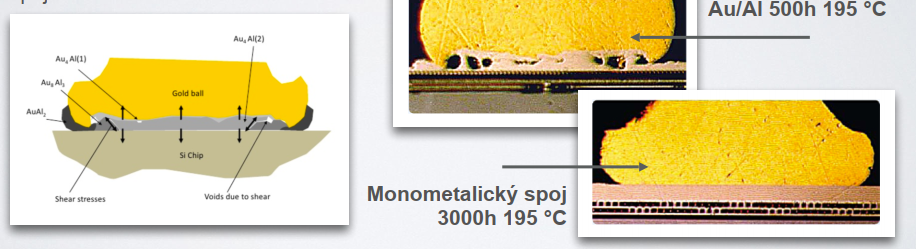
\includegraphics[scale=0.6]{images/Leach.png}
   \end{center}
   \caption{Leaching zlata}
\end{figure}

\subsection{Stříbro}
Stříbro je nejčastěji používáno v komerčních aplikacích, kde je výsledná cena důležitým faktorem. Stejně tak jako zlato je i stříbro náchylné k leachingu do SnPb pájek, ovšem s menší intenzitou. Minimalizovat tento efekt je možné pomocí niklu naneseného na povrch pájecí plošky.

\subsection{Něco navíc ke stříbru}
Stříbro má tendenci navíc k elektromigraci v případě, kdy se mezi dvěma vodiči vyskytuje elektrický potenciál (za současné přítomnosti tekuté vody).

Tento jev se vyskytuje i u jiných materiálů (Au, Pb, Sn, …), Ag je tento jev výrazně
významnější díky svému velkému ionizačnímu potenciálu.

\begin{figure}[h]
   \begin{center}
     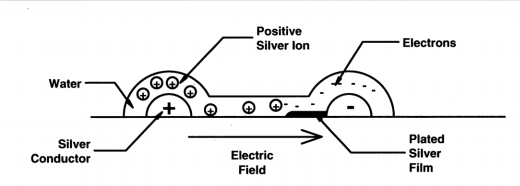
\includegraphics[scale=0.6]{images/Migrace.png}
   \end{center}
   \caption{Elektromigrace}
\end{figure}


Slitiny stříbra s paládiem a/nebo platinou vykazují jak snížení náchylnosti k leachingu, tak
náchylnosti k elektromigraci, což je předurčuje k využití v případě potřeby pájet.

Pd/Ag vodivé pasty jsou nejběžněji používané materiály v komerční oblasti TLV a hybridních
integrovaných obvodů.

Je třeba si však uvědomit, že přídavek paládia navyšuje jak cenu pasty, tak její výsledný
elektrický odpor.

Nejčastěji je proto používán poměr 4 díly Ag ku 1 dílu Pd, což poskytuje dobrý kompromis mezi
parametry pasty a její cenou.

\subsection{Význam intermetalických sloučenin v pájeném spoji}
Když reaguje pájka obsahující cín s měděným podkladem, vzniká intermetalická sloučenina Cu6Sn5, později se začne vytvářet i Cu3Sn.

Vlastnosti intermetalické fáze se liší od vlastností pájky i podkladového materiálu. Typické
pro tyto sloučeniny je vysoká křehkost a vyšší teplota tání než samotné pájky. Další významná vlastnost, zvláště v případě Cu3Sn, je nesmáčivost.

Tloušťka intermetalické fáze není statická, ale s časem roste. Rychlost růstu závisí na teplotě a růst pokračuje dokonce i při pokojové teplotě. Je-li vrstva pájky tenká, může ji intermetalická sloučenina celou nahradit a vlastnosti takovéto vrstvy se výrazně liší od té původní. Například vývod součástky pokrytý pájkou pro dosažení lepšího smočení při pájení je pokryt intermetalickou sloučeninou, která je nesmáčivá a má vyšší teplotu tání.

Mohlo by se zdát, že problémy jsou jen v případě, že upravený materiál budeme skladovat
delší dobu. Jak ale výzkum ukázal, současně s tenkou vrstvou se vytvářejí v objemu krystaly intermetalické fáze ihned po přetavení a mohou vystoupit až k povrchu. Přítomnost intermetalické fáze na povrchu mění jeho reflexivitu. Místa s intermetalickou fází jsou matná. Tento fakt by mohl způsobit problémy například s interpretací optické kontroly korektně zapájených
spojů. 


















